\documentclass{article}
\usepackage{amsmath, amssymb, amsthm, graphicx}
\usepackage[utf8]{inputenc}
\usepackage[spanish]{babel}

\title{Equivalencia de Condiciones para la Integrabilidad de Riemann}
\author{}
\date{}

\begin{document}

\maketitle

\section*{Introducción}
En el análisis matemático, la integrabilidad de Riemann es un concepto fundamental. Una función $f: [a, b] \to \mathbb{R}$ se dice Riemann integrable si existe $I \in \mathbb{R}$ tal que:
\[
\forall \epsilon > 0, \exists P \text{ partición de } [a, b] \text{ tal que } U(P, f) - L(P, f) < \epsilon.
\]
Este teorema establece condiciones necesarias y suficientes para la integrabilidad de Riemann, formuladas en tres formas equivalentes:

\begin{enumerate}
    \item \textbf{Condición de Riemann}: $\forall \epsilon > 0, \exists P$ partición de $[a, b]$ tal que $U(P, f) - L(P, f) < \epsilon$.
    \item \textbf{Condición de Darboux}: $\lim\limits_{\lVert P \rVert \to 0} U(P, f) = \lim\limits_{\lVert P \rVert \to 0} L(P, f)$.
    \item \textbf{Condición de Cauchy}: $\forall \epsilon > 0, \exists P$ partición de $[a, b]$ tal que $\forall P' \supseteq P$, se tiene $U(P', f) - L(P', f) < \epsilon$.
\end{enumerate}

\subsection*{Notación}
Sea $ P = \{ x_0, x_1, \dots, x_n \} $ una partición de $ [a, b] $, donde $ a = x_0 < x_1 < \dots < x_n = b $. Definimos la norma de la partición como
\[
\lVert P \rVert = \max_{i} (x_i - x_{i-1}).
\]
Esta cantidad mide el tamaño del subintervalo más grande en la partición.
\\
\par

La clave de estas condiciones es que, conforme el tamaño de la partición se reduce, las áreas de las barras de la suma superior e inferior se van ajustando a la misma cantidad. Intuitivamente, al hacer las particiones más finas, las oscilaciones de la función quedan cada vez más confinadas, reduciendo la diferencia $U(P, f) - L(P, f)$. Esto se puede visualizar mediante una secuencia de diagramas donde la diferencia de áreas se vuelve arbitrariamente pequeña.

\begin{center}
    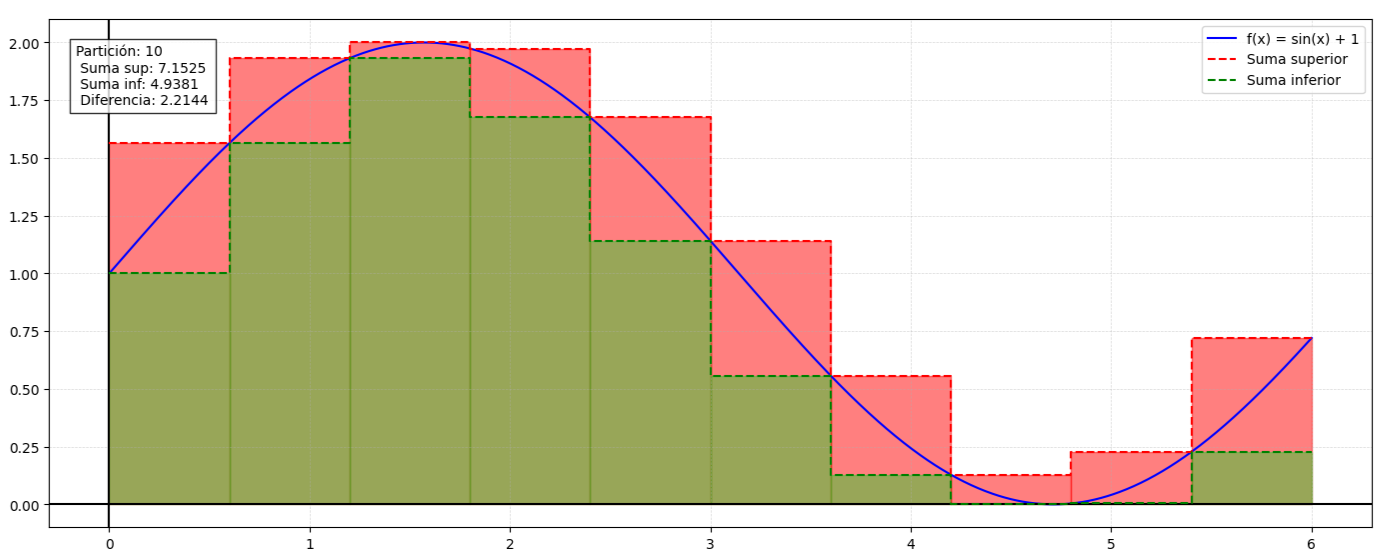
\includegraphics[width=1\textwidth]{Figure_1.png}
\end{center}

Demostraremos la equivalencia probando las siguientes implicaciones:
\[
\text{Riemann} \Rightarrow \text{Darboux} \Rightarrow \text{Cauchy} \Rightarrow \text{Riemann}.
\]

\section*{Demostración de las Implicaciones}

\subsection*{1. Riemann $\Rightarrow$ Darboux}
\textbf{Hipótesis:} $\forall \epsilon > 0, \exists P$ tal que $U(P, f) - L(P, f) < \epsilon$.

\textbf{Tesis:} $\lim\limits_{\lVert P \rVert \to 0} U(P, f) = \lim\limits_{\lVert P \rVert \to 0} L(P, f)$.

Dado $\epsilon > 0$, existe una partición $P$ tal que:
\[
U(P, f) - L(P, f) < \epsilon.
\]
Dado que $U(P, f)$ y $L(P, f)$ son respectivamente cotas superior e inferior de la integral, se tiene:
\[
L(P, f) \leq \int_a^b f(x) \mathrm{d}x \leq U(P, f).
\]
Al hacer $\lVert P \rVert \to 0$, se concluye que $U(P, f)$ y $L(P, f)$ convergen a un mismo valor, demostrando la tesis.

\subsection*{2. Darboux $\Rightarrow$ Cauchy}
\textbf{Hipótesis:} $\lim\limits_{\lVert P \rVert \to 0} U(P, f) = \lim\limits_{\lVert P \rVert \to 0} L(P, f)$.

\textbf{Tesis:} $\forall \epsilon > 0, \exists P$ tal que $\forall P' \supseteq P$, se cumple $U(P', f) - L(P', f) < \epsilon$.

Esto significa que, sin importar cómo se refinan las particiones, los valores de $U(P, f)$ y $L(P, f)$ permanecerán cercanos, asegurando la condición de Cauchy.

\begin{center}
    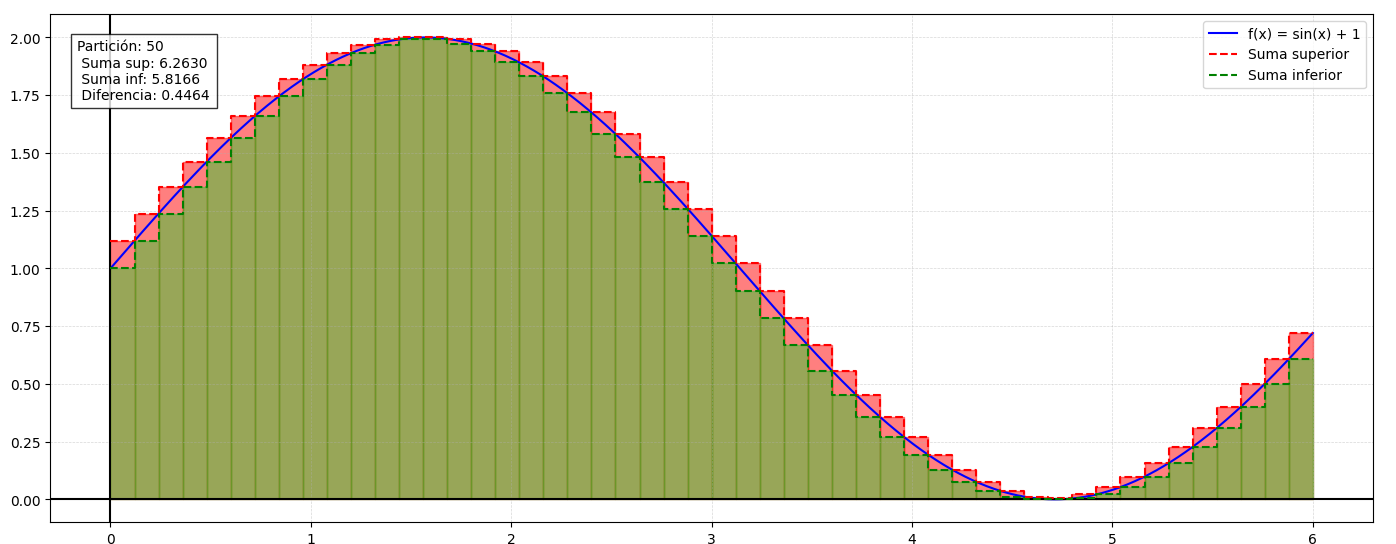
\includegraphics[width=1\textwidth]{Figure_2.png}
\end{center}

Dado $\epsilon > 0$, existe $\delta > 0$ tal que, para cualquier partición $P$ con $\lVert P \rVert < \delta$:
\[
U(P, f) - L(P, f) < \epsilon.
\]
Si $P'$ es un refinamiento de $P$, entonces $\lVert P' \rVert \leq \lVert P \rVert < \delta$, por lo que la desigualdad sigue siendo válida, demostrando la tesis.

\subsection*{3. Cauchy $\Rightarrow$ Riemann}
\textbf{Hipótesis:} $\forall \epsilon > 0, \exists P$ tal que $\forall P' \supseteq P$ se cumple $U(P', f) - L(P', f) < \epsilon$.

\textbf{Tesis:} $\forall \epsilon > 0, \exists P$ tal que $U(P, f) - L(P, f) < \epsilon$.

Este hecho implica que la función es integrable en el sentido de Riemann.

\begin{center}
    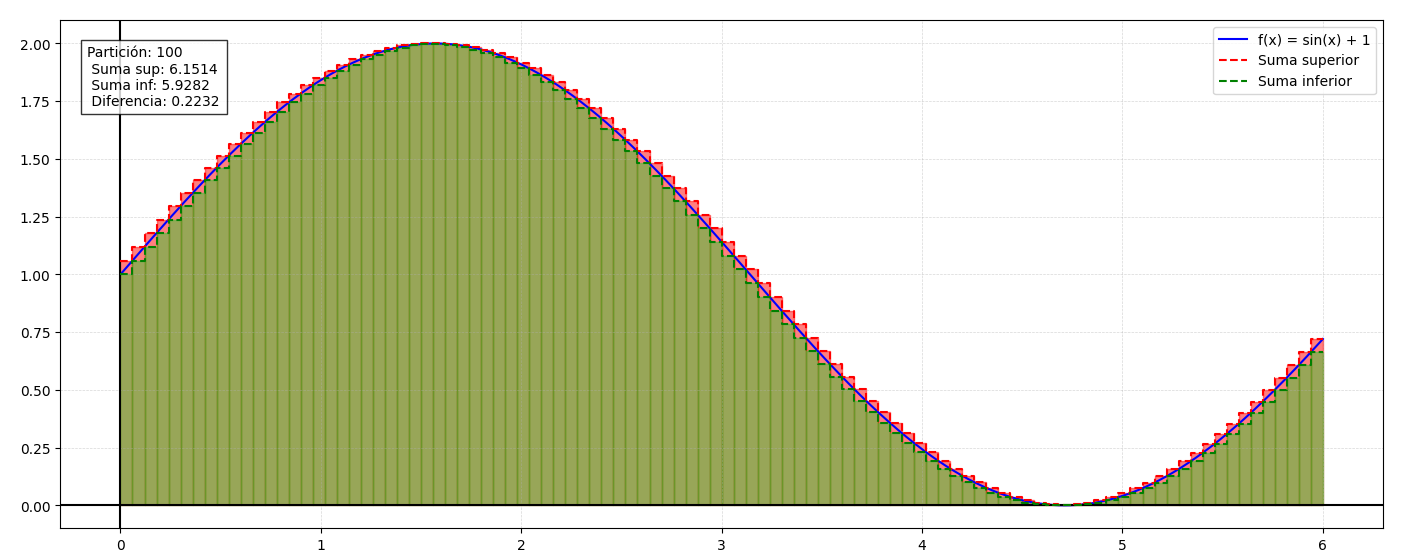
\includegraphics[width=1\textwidth]{Figure_3.png}
\end{center}

Dado $\epsilon > 0$, por la hipótesis existe una partición $P$ tal que $\forall P' \supseteq P$:
\[
U(P', f) - L(P', f) < \epsilon.
\]
En particular, tomando $P' = P$, se concluye $U(P, f) - L(P, f) < \epsilon$, demostrando la tesis.

\section*{Conclusión}
\begin{center}
    Hemos probado las implicaciones:
\end{center}
\[
\text{Riemann} \Rightarrow \text{Darboux} \Rightarrow \text{Cauchy} \Rightarrow \text{Riemann}.
\]

\begin{center}
    Por lo tanto, las tres condiciones son equivalentes:
\end{center}
\[
\text{Riemann} \iff \text{Darboux} \iff \text{Cauchy}.
\]
Esto establece que $f$ es Riemann integrable en $[a, b]$ si y solo si cumple cualquiera de estas condiciones, proporcionando un criterio riguroso para su integrabilidad.

\end{document}
